\section{Verifying the \mCTOSbase{} Kernel}
\label{sec:seq:base}

\begin{comment}
\begin{figure*}
\begin{center}
\begin{scriptsize}
\begin{tabular}{ |l|l||l|p{4.5cm}| }
  \hline
  \multicolumn{2}{|c||}{\textbf{Memory Management}} 
  & \multicolumn{2}{|c|}{\textbf{Thread and Process Management}} \\
  \hline
  \hline    
  \multicolumn{2}{|l||}{\textbf{abstract state}} 
  & \multicolumn{2}{|l|}{\textbf{abstract state}}\\
  \hline
  \verb"AT" & physical page allocation table
  & \verb"kctxp" & kernel context (\verb"kctx") pool\\
  \hline 
  \verb"PFInfo" & save the address and \verb"PC" that page fault occurs
  & \verb"Ltdqp" & low abstract thread queue pool\\
  \hline
  \verb"ptp" & page table (\verb"pt") pool 
  
  & \verb"Htdqp"& high abstract thread queue (\verb"Htdq") pool\\ 
  \hline
   \verb"ipt"& whether \verb"pt"'s invariant  should hold or not
  
  & \verb"uctxp" & user context pool\\
  \hline
\verb"PT" & index of the current \verb"pt"
  & \verb"chanp" & channel pool\\
  \hline
  \verb"pbit" & bit map for free \verb"pt" indexes
  & \verb"Htcbp"& high abstract TCB pool \\
  \hline
  \multicolumn{2}{|l||}{\textbf{primitive}} 
  & \multicolumn{2}{|l|}{\textbf{primitive}}\\
  \hline	
  \verb"setcr3" & set the starting address of the \verb"pt"
  & \verb"kctx_new" & allocate the first free \verb"pt" and \verb"kctx"\\
  \hline
  \verb"meminit" & initialize the allocation table
  & \verb"Henqueue" & append a thread to the \verb"Htdq"\\
  \hline
  \verb"palloc" & allocate a page 
  & \verb"thread_kill" & kill and free a thread\\
  \hline
  \verb"pt_insrt" & insert a page map into a given \verb"pt" 
  & \verb"thread_sleep" & sleep, schedule to the 1st ready thread\\
  \hline
  \verb"pt_resv" & allocate a page for a given linear addr 
  & \verb"kctx_switch" & switch \verb"kctx" between threads\\
  \hline 
  \verb"PTInit" & init kernel's \verb"pt" and enable paging 
  & \multirow{2}{*}{\texttt{resv\_chan}} & 
  receive msg from the channel, wake\\
  \cline{1-2}
  \verb"pt_new" & allocate the first free \verb"pt" & & up the first sleeping thread
    \\	  
  \hline
  \hline
  \multicolumn{2}{|c||}{\textbf{Virtualization}}
  &\multicolumn{2}{|c|}{\textbf{Trap Handler}} \\
  \hline
  \hline    
  \multicolumn{2}{|l||}{\textbf{abstract state}} 
  & \multicolumn{2}{|l|}{\textbf{primitive}} \\
  \hline
  \verb"npt" & nested page table for guest
  & \verb"trap_arg" & get arguments of system calls\\
  \hline
  \verb"hctx"& host context
  & \verb"hpagefault" & page fault handler\\ 
  \hline
  \verb"vmcb" & virtual machine (\verb"VM") control control block
  & \verb"sys_yield" & system calls for yielding\\
  \hline
  \verb"xvmst" & registers not saved in \verb"vmcb" 
  & \verb"sys_wait_chan" & system calls to sleep on a channel\\
  \hline
  \multicolumn{2}{|l||}{\textbf{primitive}} 
  & \verb"sys_run_vm" & system calls to run \verb"VM"\\
  \hline	
  \verb"npt_insrt" & insert into the nested page table
  & \verb"sys_proc_create" & system calls to create a process\\
  \hline
  \verb"switch2guest" &  switch to guest mode 
  & \verb"sys_getexitinfo" 
  & get the information about \verb"VM" exit\\
  \hline
  \verb"set_vmcb" & set value in virtual machine control block
  & \verb"sys_injectevent" & inject interrupt and exception to \verb"VM"\\
  \hline 
  \verb"run_vm" & save host context, restore \verb"vmcb", start \verb"VM" 
  & \verb"kernel_init" & initialization function of the kernel\\  
  \hline  

\end{tabular}
\end{scriptsize}
\caption{Key abstract states and primitives for \mCTOSbase{} and \mCTOShyper{}}
\label{table:layers}
\end{center}
\vspace*{-14pt}
\end{figure*}
\end{comment}

The \mCTOSbase{} kernel is divided into six main parts.  From the
bottom layer which corresponds to the physical machine to the top
layer providing system calls, those are the pre-initialization module
(1 layer, Section~\ref{sec:base:preinit},
Figure~\ref{fig:base:pmm:layers}), physical memory management (3 layers,
Section~\ref{sec:base:pmm}, Figure~\ref{fig:base:pmm:layers}), virtual
memory management (7 layers, Section~\ref{sec:base:vmm},
Figure~\ref{fig:base:vmm:layers}), thread management (10 layers,
Section~\ref{sec:base:tm}, Figure~\ref{fig:base:tm:layers}), process
management (4 layers, Section~\ref{sec:base:pm},
Figure~\ref{fig:base:pm:layers}), and the trap handler (3 layers,
Section~\ref{sec:base:trap}, Figure~\ref{fig:base:trap:layers}).  In
this section, we go through each module by describing its
layers from bottom to top.  

\paragraph{How to read figures describing modules}
In each figure describing a module, each rounded corner box is a layer
with the name in bold. Underneath the name is the list of abstract
states separated by commas. Primitives are enclosed in boxes
touching the bottom edge of the layer; green filling indicates
initialization primitives. Boxes filled with purple represent
a collection of primitives.

Lines with a dot on one end mark refinement relations: the box on the
flat end refines the primitive on the dotted end. On the flat end, the
box can be either a primitive, in the case of \emph{pass-through}
primitives which are implemented in layers further down in the stack,
or a function implementation (an actual piece of code) represented by
a small blue box touching the top of the layer in which it is
implemented.  A function may have outgoing arrows point to primitives
it calls (\ie, \emph{abs-fun} pattern); those without
outgoing arrows correspond to the \emph{getter-setter} pattern.

\subsection{Pre-initialization}
\label{sec:base:preinit}
The pre-initialization module only contains the bottom-most layer
\code{PreInit}, which is shown at the bottom of Figure~\ref{fig:base:pmm:layers} outside the red dashed box. It is used to model the x86 hardware and axiomatizes the
hardware behaviors that are necessary to obtain end-to-end behaviors
across the kernel and the user space. These behaviors include page
table walk upon memory load when paging is turned on, 
address save during the page fault,
and the mode change made by the ring switch.
\ignore{
The \code{x86} object is the only layer object in the \code{PreInit} layer.
It extends the CompCert assembly semantics
to model the low-level features of the machine.}
Its abstract state consists of a kernel mode flag \code{ikern},
an initialization flag \code{init},
a physical memory map \code{MM},
and control registers.
Its primitives consist of
a function modeling the transition between user and kernel mode,
and 
getter-setter functions for control registers and \code{MM}.

\paragraph{Kernel mode} The logical flag \code{ikern} indicates
whether the processor is currently in kernel or user mode.
The \code{kernel\_mode} predicate of \code{PreInit}
is defined as $``\code{ikern} =\code{true}"$.
Actually, all the sequential layers for \mCTOS{} use the same
 \code{kernel\_mode} predicate
 (\mCTOShyper{} uses a different one).
Some privileged
memory regions (\eg, allocation table) and 
instructions (\eg, modifying control registers)
are only available in kernel mode.
\ignore{
The switch function models the change of the \code{ikern} flag
and the remaining tasks involved with trap handling,
such as saving and restoring user and kernel contexts,
and dispatch over the trap type,
are verified at the assembly level.
}



\paragraph{Initialization primitive}
$\code{preinit}$
at this bottom-most layer models the bootloader,
which initializes \code{MM} and necessary drivers
(\eg, timer, keyboard, serial, {\it etc.}),
loads the kernel into the memory,
and sets the initialization flag $\code{init}$ to be \code{true}.
The state component \code{MM} is the abstraction of the
E820 memory map provided by the bootloader.
It can be accessed only when 
$\code{init}$ is $\code{true}$.

\paragraph{Memory accessor} 
The control registers \code{CR0}, \code{CR2},  \code{CR3},
and \code{OEIP}
(a pseudo-register to save the \emph{old $\code{EIP}$} when an exception happens
)
are used to model the behavior
of the processor's memory management unit (MMU),
which is specified by the \emph{memory accessors}
of \code{PreInit}.
The rules for the load accessor are shown below
(the store accessor ones are similar).

\begin{mathpar}
\inferrule{ 
a.\code{CR0} = \code{false}
}{ \Gamma \vdash\code{PreInit}.\mat.load(v; \rho, m, a)  = (m(v); \rho, m, a)}
\and
\inferrule{ 
a.\code{CR0} = \code{true}
\\
\code{addr\_trans}(a,v) = \some{v'}
}{ \Gamma \vdash\code{PreInit}.\mat.load(v; \rho, m, a)  = (m(v'); \rho, m, a)}
\and
\inferrule{ a.\code{CR0} = \code{true}
\\
\code{addr\_trans}(a,v) = \None\\
a' = a \set{\code{CR2}: v}\set{\code{OEIP}: \rho(\code{EIP})}\\
\rho' = \rho\set{\code{EIP}: (\Gamma(\code{PF\_handler}),0)}
}{ \Gamma \vdash\code{PreInit}.\mat.load(v; \rho, m, a)  = (\cdot; \rho', m, a')}
\end{mathpar}
When paging is enabled (as indicated by \code{CR0}),
memory accesses (\ie, load and store) made by both the kernel and the user programs
are translated using the page map pointed to by \code{CR3}.
The address translation function
$\code{addr\_trans}$ is
shown in Figure~\ref{fig:seq:mem1}.
When a page fault occurs,
the corresponding information is stored in \code{CR2}
and \code{OEIP},
and then the page fault handler $\code{PF\_handler}$ is invoked.

\paragraph{Layer invariant}
To make sure that it is safe to compile
kernel code with CompCertX,
we have to show that, in the kernel mode,
the memory accessors are equal to the CompCert accessors
(\cf Section~\ref{sec:seq:comp:concrete}).
It is stated as a layer invariant of \code{PreInit}.
\begin{invariant}[Valid memory accessors]
If $a.\code{CR0} = \code{true}$
and $a.\code{ikern} = \code{true}$,
we have $\code{addr\_trans}(a,v) = \some{v}$,
 meaning that the address translation is identity.
\end{invariant}

To prove this invariant holds for \code{PreInit},
we have to add pre-conditions
to the primitives that change $\code{CR0}$ and $\code{CR3}$
registers:
1) paging is enabled only if this invariant
holds;
and 2) in the kernel mode,
the page table pointed by $\code{CR3}$
has to be an identity map
after paging is enabled.
At upper layers,
we  show that
these pre-conditions
are satisfied
when invoking setter primitives for $\code{CR0}$ and $\code{CR3}$.

What's more,
we also need an invariant that there is enough
physical memory to boot \mCTOS{}.
Currently, we set 1GB as the minimal requirement,
and all the kernel code and data are stored below
1GB. The actual memory usage of \mCTOS{}
is much less than this requirement.
\begin{invariant}[Enough memory space]
If $a.\code{init} = \code{true}$,
the memory space indicated by $a.\code{MM}$
is within the range
$[1GB, 4GB]$.
\end{invariant}

\begin{figure*}[t]\centering
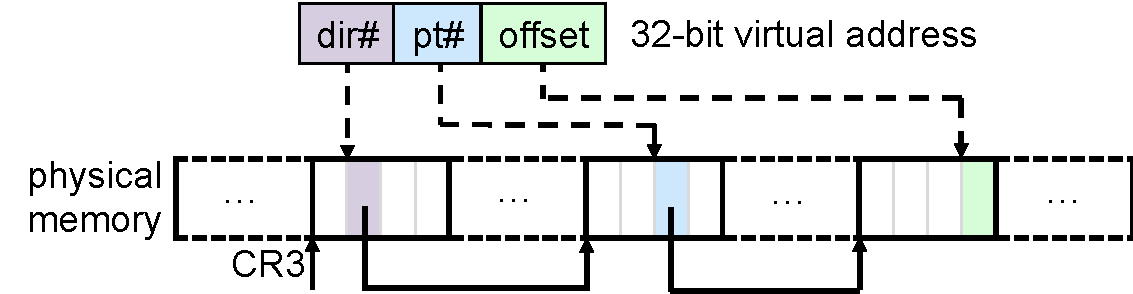
\includegraphics[scale=.55]{figs/mem_model_1} 
\caption{Address translation at \code{PreInit} layer}
\label{fig:seq:mem1}
\hrulefill
\end{figure*}




\subsection{Physical memory management}
\label{sec:base:pmm} 

{
\begin{figure}\centering
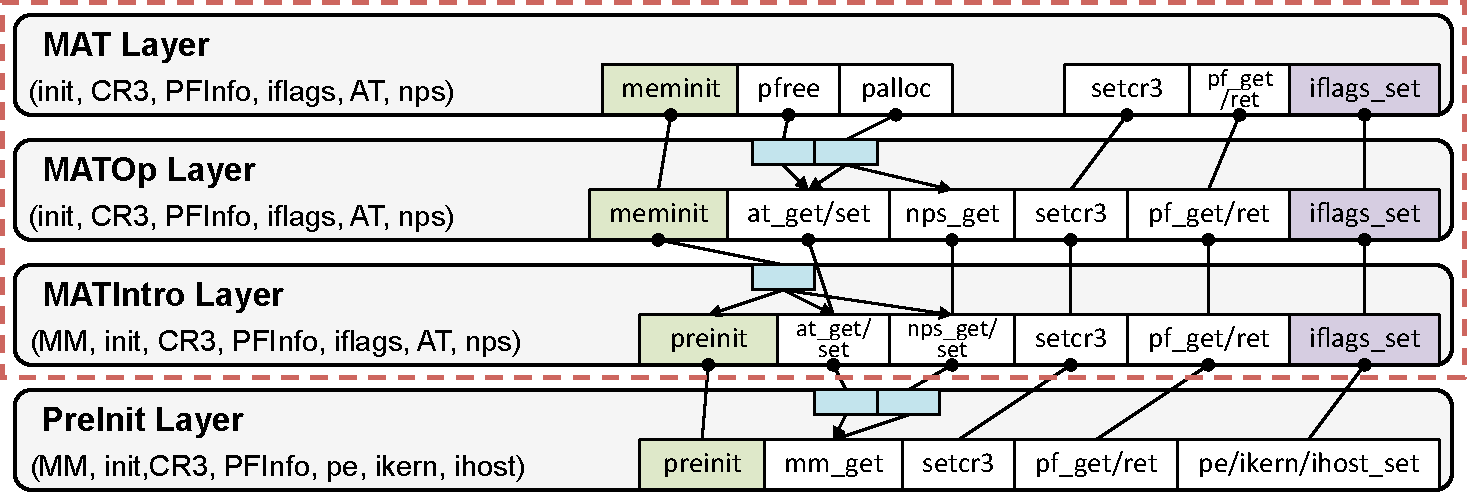
\includegraphics[scale=0.5]{figs/pmm_layer}	
\caption{Layers of physical memory management}
\label{fig:base:pmm:layers}
\hrulefill
\end{figure}
}

Based on the pre-initialization layer and its memory
accessors,
the physical memory management introduces the physical page,
which supports dynamic allocation.
To better reason about access control and isolation in the case of
the dynamic resource allocation, each physical page
object maintains a \emph{logical} state containing ownership information,
and the page is only allowed to be accessed by its owners.

The physical memory management of \mCTOSbase{}
consists of  3 layers, which are shown in the red dashed box in
Figure~\ref{fig:base:pmm:layers}.
The module introduces three new abstract states: 
\code{nps} (the number
of physical pages),
\code{AT} (the page allocation table
indicating the physical page information),
and \code{cn} (the page usage of each thread).  

\paragraph{Layer hierarchy}
Layer $\code{MATIntro}$
introduces the getter-setter methods
for these newly introduced abstract states.
These states are initialized by \code{meminit} using the information
stored in \code{MM}, provided by the layer
$\code{MATInit}$. 
Besides this initialization primitive,
the topmost layer $\code{MAT}$ in this module
also exports two more primitives
\code{palloc} and \code{pfree},
which allocate and free physical pages,
respectively.

\begin{figure}[t]
\lstinputlisting [language = C, multicols=2] {source_code/seq-palloc2.c}
\caption{Pseudocode of \texttt{palloc} in \mCTOS{}}
\label{fig:seq:palloc}
\hrulefill
\end{figure}

\ignore{
The module first
defines a getter-setter layer \verb"MATIntro", followed by an
abs-kernel-fun layer \verb"MATOp" where a new initializer is defined,
and then another abs-kernel-fun layer \verb"MAT" which provides the
physical page allocator.
}

\paragraph{Enforcing memory quotas}
One important function of the physical memory management is to dynamically
track and bound the memory usage of each thread. A \emph{container}
object $\code{cn}$ is used to record information for each thread (represented as the array \code{cn}
in Figure~\ref{fig:seq:palloc}); one piece of information tracked is the
thread's \emph{quota}. Inspired by the notions of containers and
quotas in HiStar~\cite{zeldovich06}, a thread
in {\mCTOS} is spawned with some quota specifying the maximum number
of pages that the thread will ever be allowed to allocate. As can be
seen in Figure~\ref{fig:seq:palloc}, \code{palloc} returns an error
code if the requesting thread has no remaining quota (lines~2 and 3), 
and the quota is decremented when a page is successfully allocated (line~14).
Quota enforcement allows the kernel to prevent a denial-of-service attack,
where one thread repeatedly allocates pages and uses up all available
memory (thus denying other threads from allocating pages). From a security
standpoint, it also prevents the undesirable information channel between 
different threads that occurs due to such an attack.

\paragraph{Page management}
Section~\ref{sec:clightx-prog}
already provides
a detailed procedure
to build layers for a simplified version of
$\code{palloc}$.
The design pattern
is shared for most of the primitives:
first introducing getter-setter methods,
and hiding the concrete memory;
then verifying the primitive using
getter-setter methods.
To improve
readability,
in the rest of this thesis,
we will omit
this design pattern,
and only show the primitives' specifications
in terms of inference rules.
For example,
the rules for $\code{palloc}$ primitive are shown as below.
\begin{mathpar}
\inferrule{
q = a.\code{cn}(\ttid).\code{quota} \ge 1 \\
0 \le \mathit{freei} < a.\code{nps}\\ 
a.\code{AT}(\mathit{freei}).\code{is\_alloc} = \false \\
\forall 0 \le i < \mathit{freei}, a.\code{AT}(i).\code{is\_alloc} = \true \\
a' = a \set{\code{AT},\mathit{freei}: (\true, 1,\ttid, \code{freeable})}
\set{\code{cn}.\code{quota},\ttid: q - 1}
}{
\Gamma  \vdash  \spec_{\code{palloc}}([\ttid],m, a, \mathit{freei}, m, a')
}
\and
\inferrule{
(a.\code{cn}(\ttid).\code{quota} < 1)
\vee
(\forall 0 \le i < a.\code{nps}, a.\code{AT}(i).\code{is\_alloc} = \true)
}{
\Gamma  \vdash  \spec_{\code{palloc}}([\ttid],m, a, \error, m, a)
}
\end{mathpar}
Each entry of the allocation table is a tuple
$(\code{is\_alloc}, \code{ref}, \code{owner}, \code{status})$,
where $(\code{is\_alloc}:\code{bool})$ indicates
if the page is allocated or not,
$\code{ref}$ is the number of references to the page,
$\code{owner}$ is the page owner,
and $\code{status}$ stores the page status
(\eg, $\code{freeable}$ and $\code{writable}$).

\paragraph{Layer invariant}
Since the allocation table is set up using $\code{MM}$,
we have to guarantee that these two tables
are consistent.
\begin{invariant}[Valid physical memory management]
If $a.\code{init} = \code{true}$,
we have 
1) $2^{18} \le a.\code{nps} \le 2^{20}$;
2) $\forall 0 \le i \le 2^{18},  a.\code{AT}(i).\code{is\_alloc} = \true$ (i.e., reserved for the kernel);
and 3) for any invalid page $i$ indicated by $a.\code{MM}$
(e.g., reserved for devices),
$a.\code{AT}(i).\code{is\_alloc} = \true$.
\end{invariant}

\ignore{
\paragraph{Enforcing memory quotas}

Another function of the physical memory management is to dynamically
track and bound the memory usage (in terms of number of dynamically-allocated
pages) of processes based on their id.

In \mCTOSbase{}, we consider every unique
integer (up to some predefined maximum, currently $2^{18}$) to represent
a different agent or principal. We refer to this integer as the agent's
id, and we use it for all layer objects owned by that agent. % For example,
% whenever \mCTOSbase{} receives a request to spawn a process, it picks some 
% currently unused id $i$ and creates a new container, page map, and thread 
% control block, all of which are bound to the same id $i$. Thus
% The id serves
% as a simple and global way to relate various kernel objects to a single agent.


The MContainer layer introduces a notion of container, inspired by container 
objects in the HiStar operating system~\cite{zeldovich06}. 
Whenever a new agent (id) is created in \mCTOSbase{}, a container is created for the agent 
that dynamically keeps track of its memory usage. 
An agent's usage may increase for a few reasons, including a direct request for 
dynamically-allocated resources, or a successfully-handled page fault. Each container 
object is initialized with some maximum \emph{quota}; any attempt for an agent to increase 
its usage beyond this quota will be denied by the kernel. Furthermore, the kernel maintains a mapping of ids to containers using
a hierarchical tree structure. Whenever an agent's process makes a request to spawn a
new process, the new container is added as a child to the requesting agent's container,
and the new container's quota is taken from the requester's.

With this notion of container, we are able to prove a theorem about reliability of 
dynamic memory allocation: agents' requests for additional resources will always be 
fulfilled as long as their quota is not exceeded.
Furthermore, from the viewpoint of information-flow security, resource quotas close the 
potential for two different processes to communicate via allocation requests.
Hence quota enforcement provides an additional level of security for \mCTOSbase{}.
%
We plan to extend the concept of containers to other types of
resources in the future. For example, we could maintain a time-slice quota
for each agent.  This would provide a foundation for reasoning about
liveness properties for processes and security breaches via timing
channels.}


\ignore{
To verify the implementations of \verb"palloc" and \verb"pfree",
we prove the following invariant at layer \verb"MATOp".
\begin{invariant}
\label{inv:atable}
After the initialization (\verb"init" = \verb"true"),
(1) $2^{18} \le \verb"nps" < 2^{20}$, (2) physical page in low memory part has type \verb"PG_KERNEL", and
(3) physical page in high memory part has type \verb"PG_KERNEL" or \verb"PG_NORMAL".
\end{invariant}

\begin{figure}[ht]\scriptsize
$$
\begin{array}{l|l}
\begin{array}{l}
\verb"typedef enum {"\\
\verb"  PG_RESERVED,"\\
\verb"  PG_KERNEL,"\\
\verb"  PG_NORMAL"\\
\verb"} pg_type;"\\
\\
\verb"struct pginfo {"\\
\verb"  pg_type	t;"\\
\verb"  int	used;"\\
\verb"};"\\
\\
\verb"struct pginfo AT[1<<20];"
\end{array}
&
\begin{array}{l}
\verb+Inductive pg_type :=+\\
\verb+| PG_RESERVED+\\  
\verb+| PG_KERNEL+\\  
\verb+| PG_NORMAL.+\\
\\
\verb+Inductive pginfo :=+\\
\verb+| ATValid (t: pg_type)+\\
\verb+          (used: bool)+\\ 
\verb+| ATUndef.+\\
\\
\verb+Definition AT :=+\\
\verb+      ZMap.t pginfo.+\\
\end{array}
\\\vspace*{-14pt}
\end{array}
$$ 
\caption{Concrete vs. abstract page allocation table}
\label{fig:abs:atable}
\vspace*{-14pt}
\end{figure}

}


\subsection{Virtual memory management}
\label{sec:base:vmm} 

\begin{figure}\centering
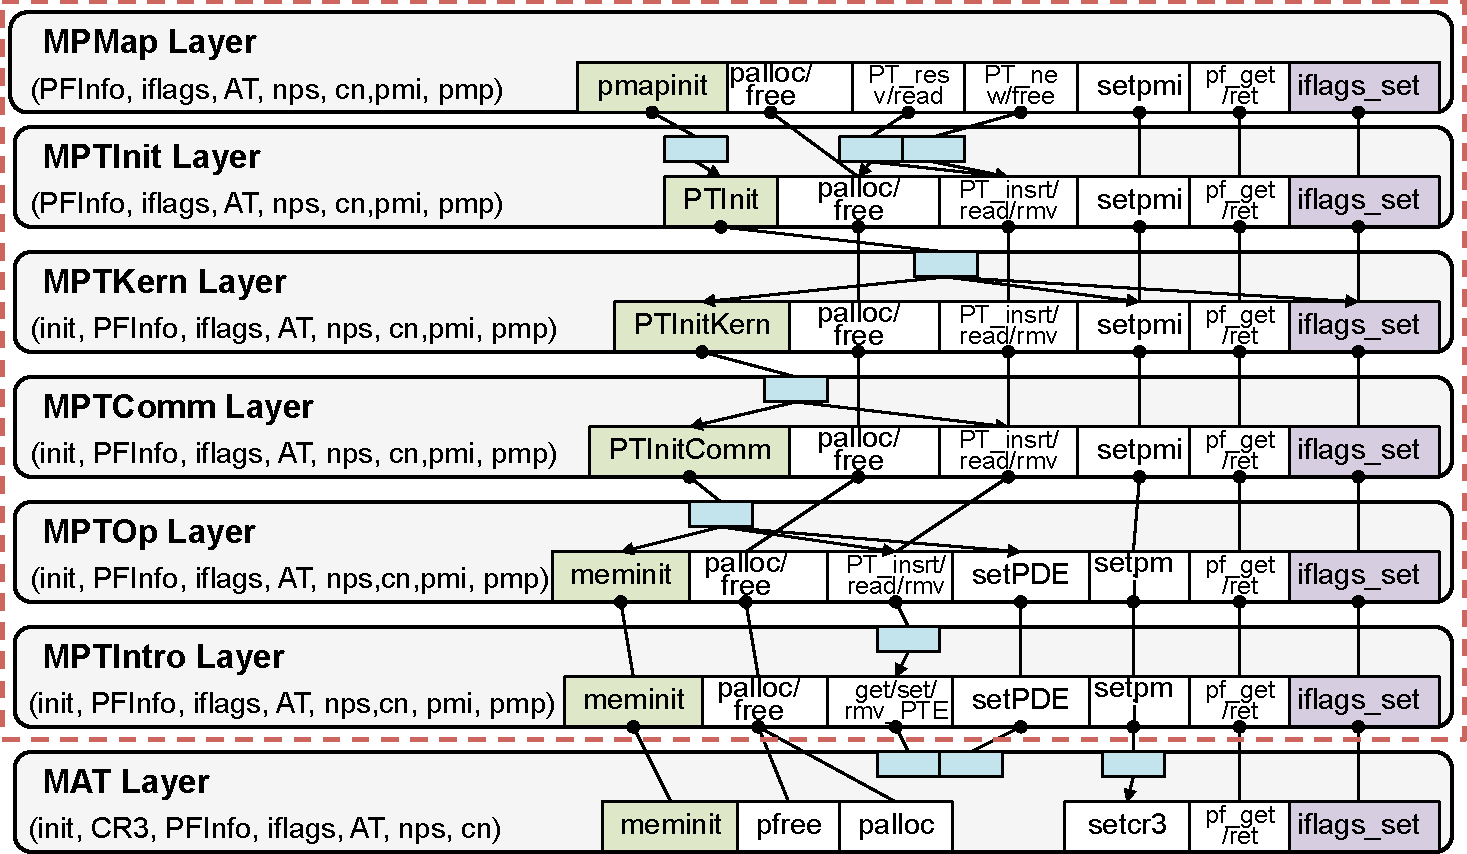
\includegraphics[scale=0.5]{figs/vmm_layer}	
\caption{Layers of virtual memory management}
\label{fig:base:vmm:layers}
\hrulefill
\end{figure}

\ignore{
We still focus on memory in the next module, however, we turn our
attention to user programs' needs.  
}
On top of physical memory management,
the virtual memory management implements
the two-level \emph{page map}, which
provides consecutive virtual address spaces.

\paragraph{Layer hierarchy}
As shown in
Figure~\ref{fig:base:vmm:layers}, the virtual memory management of
\mCTOSbase{} consists of 6 layers: 1) getter-setter layer \verb"MPTIntro"
defines two new abstract states, the page map pool \verb"pmp" (which
consists of 73 page tables) and the page map index \verb"pmi" (which
points to the current page table); 
2) abs-kernel-fun layer \verb"MPTOp"
introduces primitives to access page maps including \verb"pt_insrt" and \verb"pt_read"; 3) the following three abs-kernel-fun layers
\verb"MPTComm", \verb"MPTKern", and \verb"MPTInit" build the
initialization primitive \verb"PTInit" to initialize the page map pool;
and 4) abs-kernel-fun layer \verb"MPMap" 
provides wrapper primitives
for a user process to allocate a page and insert to its page map.



\paragraph{Memory accessor}

\begin{figure}[t]\centering
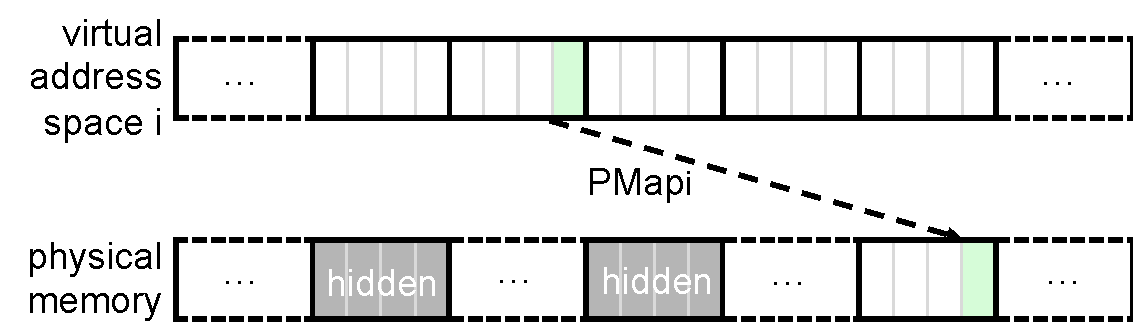
\includegraphics[scale=.55]{figs/mem_model_2} 
\caption{Address translation at \code{MPTInit} layer}
\label{fig:seq:mem2}
\hrulefill
\end{figure}

Starting from the \verb"MPTIntro" layer, we 
introduce new memory accessors
using page maps.
As shown in Figure~\ref{fig:seq:mem2},
the
address translation $\code{pm\_addr\_trans}$ at this layer is defined
using \verb"pmp" and \verb"pmi" instead of the physical two-level page
table and the \verb"CR3" register. 

The page map pool $(\code{pmp}: \integer\partialf \code{pm})$
is a partial function from the page map index $\code{pmi}$
to a map $\code{pm}$.
The  two-level page map $(\code{pm} : \integer\partialf \code{pde})$
is a partial function  from page index to a pair 
$(\code{pde}, \code{pde\_loc})$.
The page directory entry 
$\code{pde}$
is a partial function from page index to a page table entry
$\code{pte}:=(\mathit{vadr}, \mathit{perm})$.
The physical page storing
the page directory entry is represented
as $\code{pde\_loc}$.

The address translation walks through
the page map and returns the page table entry if it exists.
We write $a.\code{pmp}(a.\code{pmi})$ as a function to walk
through the page map.
Thus, the address translation function is shown as below.
\begin{mathpar}
\inferrule{
a.\code{pmp}(a.\code{pmi})(v/\code{PgSize}) = \some{(i, p)} \\
\code{perm\_allow}(a.\code{ikern}, p) \\
v' = i \times \code{PgSize} + (v\ \code{mod}\  \code{PgSize})
 }{\code{pm\_addr\_trans} (a, v) = \some{v'}}
\end{mathpar}
It first acquires the virtual page index and the page permission
from the page map,
then checks the permission,
and finally translates the physical address
to the virtual address.
The default page size $\code{PgSize}$ is 4KB.
Thus, the memory accessors of \code{MPTIntro} is defined
using $\code{pm\_addr\_trans}$, instead of
$\code{addr\_trans}$ used in \code{PreInit}.
 The contextual refinement relation
between these two kinds of memory accessors guarantees that the
value in the \verb"CR3" register is always a valid starting address of
a well-formed page table.



\paragraph{Page map operation}

\begin{figure}[t]\centering
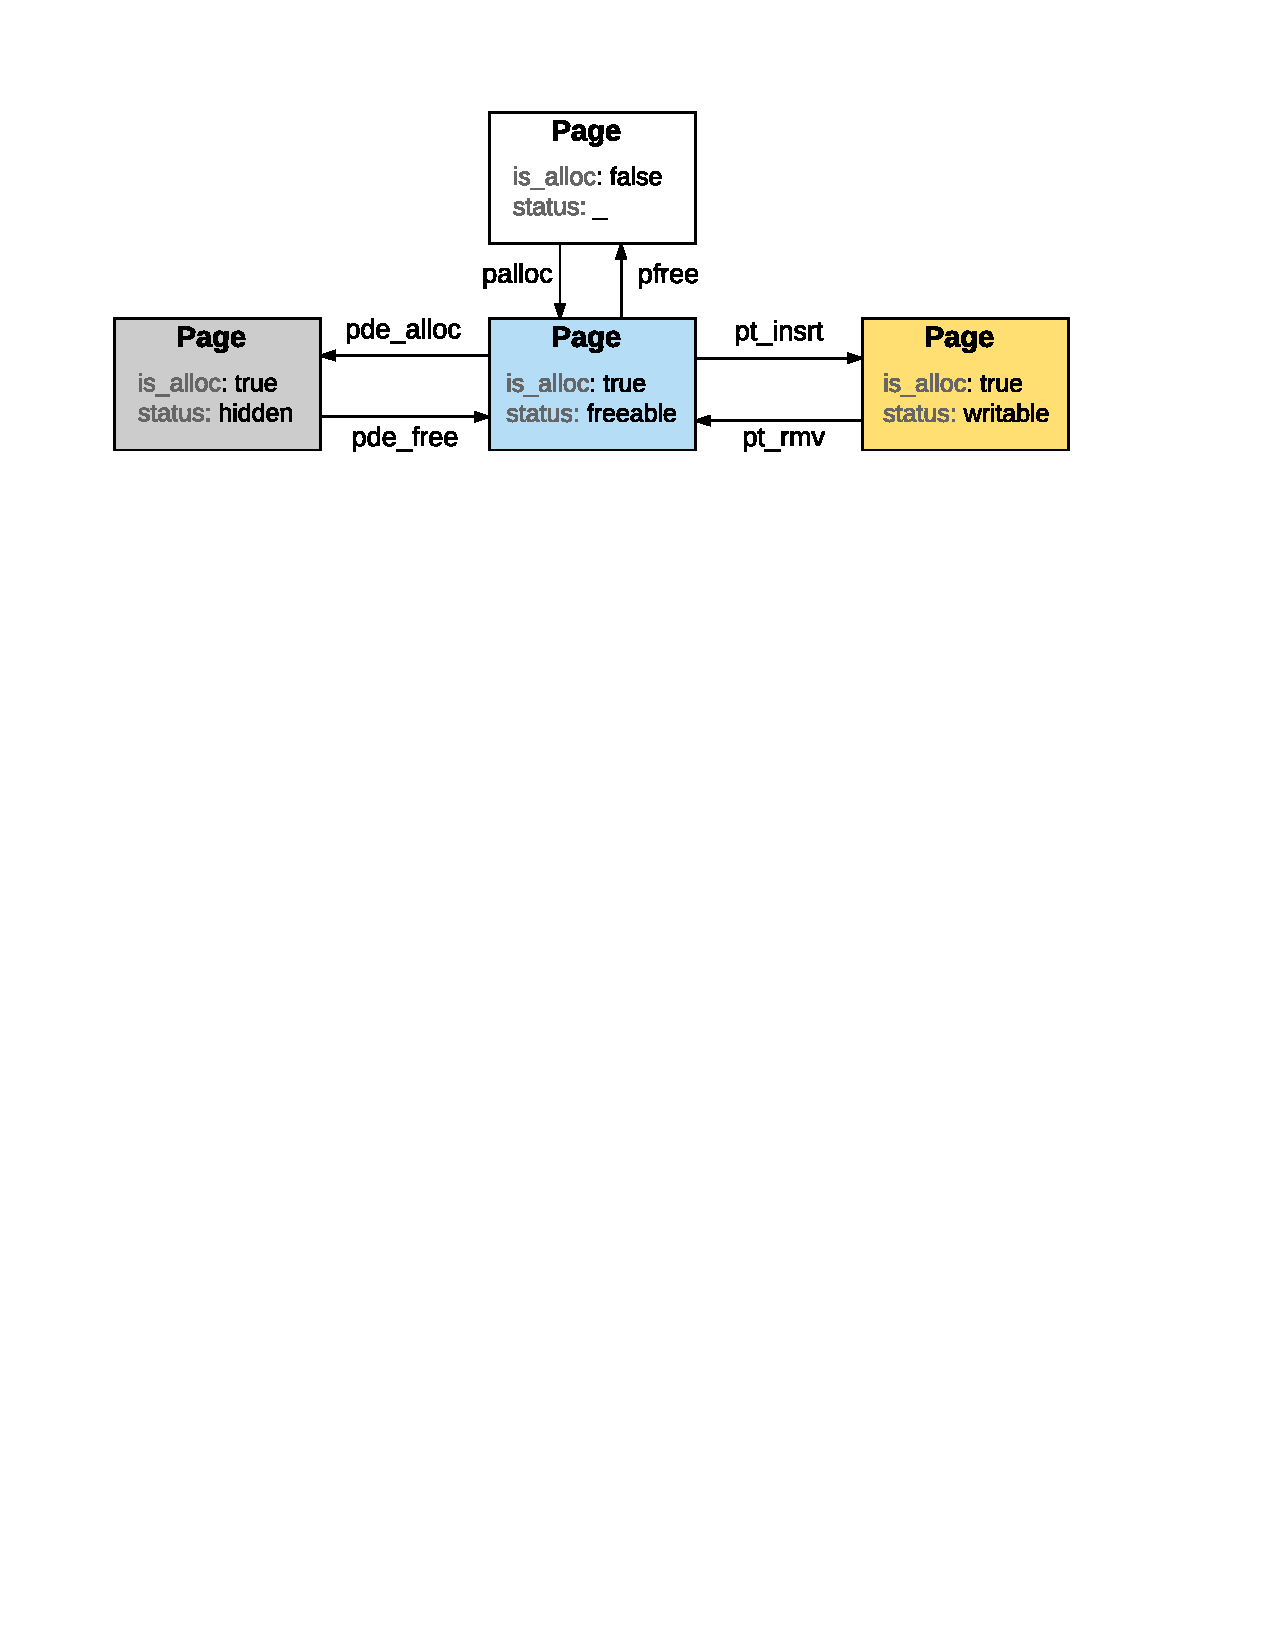
\includegraphics[scale=.8]{figs/page_status} 
\caption{The state of page status related to page map}
\label{fig:seq:pages}
\hrulefill
\end{figure}

In \mCTOS{},
we statically reserve one page (\ie, 4KB)
for each process to store  the first-level page table
(\ie, page directory).
The second-level page table (\ie, pointed by page directory entry)
is dynamically allocated
using $\code{pde\_alloc}$.
It first allocates a free page,
turns the page into an abstract page table,
and sets the page status to be $\code{hidden}$ (\cf Figure~\ref{fig:seq:pages}).
\begin{mathpar}
\inferrule{
\Gamma  \vdash  \spec_{\code{palloc}}([\ttid],m, a, \mathit{freei}, m, a_0)\\
\mathit{freei} \neq \error \\
a' = a_0\set{\code{pmp}, \ttid, \mathit{vpi}: (\emptyset, \mathit{freei})}
\set{\code{AT}, \mathit{freei}: (\true, 1,\ttid, \code{hidden})}
}{
\Gamma  \vdash  \spec_{\code{pde\_alloc}}([\ttid\cons \mathit{vpi}],m, a, \mathit{freei}, m, a')
}
\and
\inferrule{
\Gamma  \vdash  \spec_{\code{palloc}}([\ttid],m, a, \error, m, a)
}{
\Gamma  \vdash  \spec_{\code{pde\_alloc}}([\ttid\cons \mathit{vpi}],m, a, \error, m, a)
}
\end{mathpar}
By setting the page status, the page contents can only be accessed
by the page map primitives,
instead of the regular memory manipulations.
Different from the CompCert memory 
permission,
this page status is purely logical,
and is organized in terms of the physical page
rather than the CompCert memory block.

To insert
a virtual and physical page index pair
$(\mathit{vpi}, \mathit{ppi})$ to the page map,
$\code{pt\_insrt}$ has to guarantee that
the second-level page table for $\mathit{vpi}$ 
is present,
and the physical page $\mathit{ppi}$ has already been
allocated.
Then, the page status of $\mathit{ppi}$ is changed
to $\code{writable}$,
meaning that the page is writable through
memory operations,
but cannot be freed by $\code{pfree}$
primitive (\cf Figure~\ref{fig:seq:pages}).
 \begin{mathpar}
\inferrule{
a.\code{pmp}(tid)(\mathit{vpi}) = (\mathit{pde}, i)\\
\mathit{pde}' = \mathit{pde}\set{\mathit{vpi}: (\mathit{ppi}, p)} \\
a.\code{AT}(\mathit{ppi}) = (\true, r,\ttid, \code{freeable}) \\
a' = a\set{\code{pmp}, \mathit{vpi}: (\mathit{pde}' , i)}
\set{\code{AT}, \mathit{ppi}: (\true, r,\ttid, \code{writable})}
}{
\Gamma  \vdash  \spec_{\code{pt\_insrt}}([\mathit{tid}\cons \mathit{vpi}\cons \mathit{ppi} \cons p],m, a, \cdot, m, a')
}
\end{mathpar}

\paragraph{Initialization primitive}
We proved not only that the primitives of virtual memory management
manipulate the address space correctly,
but also that the initialization procedure sets up the two-level page maps properly
in terms of hardware address translation.
After paging is enabled, both kernel modules and user processes
run in a virtual address space.
To ensure the correctness of these kernel modules and user processes on top of virtual memory
management, we prove the following invariants:
\begin{invariant}
\label{inv:seq:virtual}
1) paging is enabled only after the initialization of virtual memory management;
2) if $a.\code{init} =\true$, the memory regions (i.e., lower 1GB) that store kernel-specific data must have the kernel-only 
permission in all page maps;
3) if $a.\code{init} =\true \wedge a.\code{ikern} =\true $, 
the current page map $a.\code{pmp}(a.\code{pmi})$
is an identity map.
\end{invariant}

Invariant~\ref{inv:seq:virtual} no longer holds 
if the privileged primitive that sets the \code{CR3}
register is present in the layer, as the unknown context code may write
an invalid address into \code{CR3} using the provided primitive. To solve this issue, 
the $\code{MPTIntro}$
layer is introduced with a wrapper function 
$\code{setpmi}$
that takes the process $id$ as argument,
instead of an actual address. Then the function sets \code{CR3} to the
starting address of the predefined corresponding process's page table structure.
The primitive $\code{setcr3}$ that directly sets the \code{CR3} register is hidden from the
new layer, and the invariants are introduced in this layer.
This is one of the rare cases where performance overhead is introduced
(one extra function call due to the wrapper).
It is possible to use CompCertX's function-inlining optimization
to remove this overhead, which is left as future work (\cf Section~\ref{chap-limits}).

\subsection{The shared memory management} 
In \mCTOS{}, the shared memory management provides a protocol to share physical
pages among different user processes. 
It provides an infrastructure to map a physical page into multiple
processes' page maps in different address spaces.
Our ownership mechanism ensures that the page can only be freed once 
all processes release ownership.

\ignore{
\begin{figure}[ht]\scriptsize
$$
\begin{array}{l|l}
\begin{array}{l}
\verb"#define PDES    1024"\\	
\verb"#define PTES    1024"\\
\verb"#define PTEP    0x001"\\
\verb"#define PTEW    0x002"\\
\verb"#define PTEU    0x004"\\
\\
\verb"struct pmap {"\\
\verb"  uint32_t pd[PDES];"\\
\verb"  uint32_t pt[PDES][PTES];"\\
\verb"};"\\
\\
\verb"struct pmap pmp[64];"
\end{array}
&
\begin{array}{l}
\verb+Inductive PTPerm :=+\\
\verb+| PTEP | PTEW | PTEU.+\\
\verb+Inductive PTE:=+\\
\verb+| PTEV (v: block)+\\
\verb+       (p: PTPerm)+\\
\verb+| PTEUnPresent+\\
\verb+| PTEUndef.+\\
\verb+Definition PT :=+\\
\verb+      ZMap.t PTE.+\\
\verb+Inductive PDE :=+\\
\verb+| PDEV (pt: PT)+\\
\verb+| PDEUndef.+\\
\verb+Definition pmap :=+\\
\verb+      ZMap.t PDE.+\\
\verb+Definition pmp :=+\\
\verb+      ZMap.t pmap.+
\end{array}
\\\vspace*{-14pt}
\end{array}
$$ 
\caption{Concrete vs. abstract page table}
\label{fig:abs:ptable}
\end{figure}

Since \verb"PTInit"  enables paging after initializing \verb"pmp", the addressing mode changes inside the function execution. Therefore, verification of the initialization function need to enforce that:
\begin{invariant}
\label{inv:pagemap}
When paging is enabled (\verb"pe" = \verb"true"),
(1) the low memory part of all page maps in \verb"pmp" must be identity maps, and
(2) if in the kernel mode (\verb"kern" = \verb"true"), the current page table (\verb"pmp[pmi]") must be an identity map.
\end{invariant}
}


\subsection{Thread management}
\label{sec:base:tm} 

{
\begin{figure}\centering
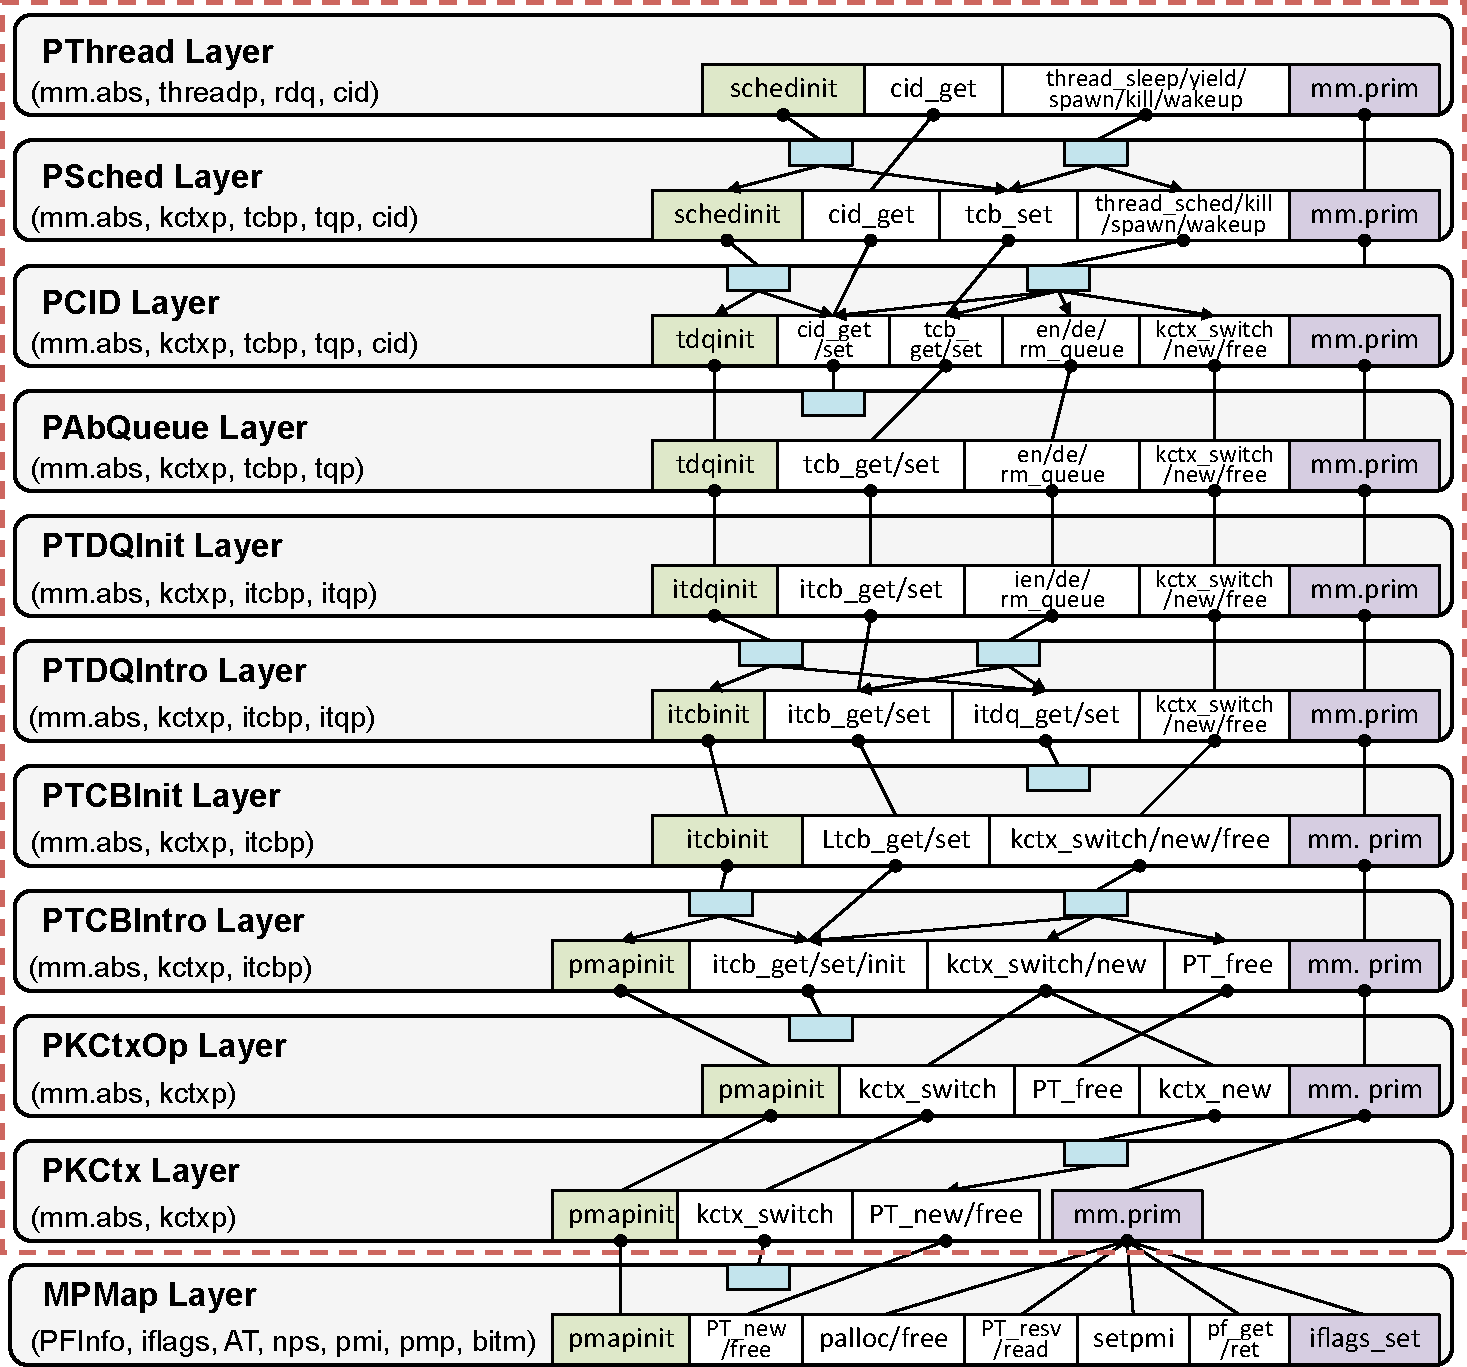
\includegraphics[scale=0.5]{figs/tm_layer}	
\caption{Layers of thread management}
\label{fig:base:tm:layers}
\hrulefill
\end{figure}
}

\ignore{
\begin{figure}[ht]\scriptsize
$$
\begin{array}{l|l}
\begin{array}{l}
\verb+Record thread := {+\\
\verb+  id: Z;+\\ 
\verb+  kernel_context: kctx;+\\
\verb+  TCB: tcb;+\\
\verb+  sleep_queue: tdq+\\
\verb+}+
\end{array}
&
\begin{array}{l}
\verb+Record process := {+\\
\verb+  td: thread;+\\
\verb+  pagemap: pmap;+\\
\verb+  user_context: uctx;+\\
\verb+  channel: chan+\\
\verb+}+
\end{array}
\\\vspace*{-14pt}
\end{array}
$$ 
\caption{Abstract thread and process}
\label{fig:abs:threadproc}
\end{figure}
}


The thread management module consists of 10 layers and is
shown in Figure~\ref{fig:base:tm:layers}.  The layers \verb"PKCtx",
\verb"PTCBIntro", and \verb"PTDQIntro" are getter-setter layers
defining the kernel context pool \verb"kctxp", the intermediate
abstract thread control block (TCB) pool \verb"itcbp", and the
intermediate thread queue pool \verb"itdqp", respectively, while
\verb"PKCtxOp", \verb"PTCBInit", and \verb"PTDQInit" are
abs-kernel-fun layers introducing operations over these abstract
states. The top four layers then finalize the abstraction into the
thread pool \verb"threadp", the ready queue \verb"rdq", and the
current thread id \verb"cid", and provide the standard thread
primitives such as \verb"thread_spawn" and \verb"thread_yield".
\ignore{
{
\setlength{\floatsep}{-10pt}
\setlength{\belowcaptionskip}{-10pt}
\vspace*{-10pt}
\begin{figure}[ht]\tiny
$$
\begin{array}{l|l}
\begin{array}{l}
\verb+struct tcb *+\\
\verb+dequeue(struct tdq * queue){+\\
\verb+  struct tcb * head, next;+\\
\verb+  struct tcb * pid = null;+\\
\verb+  if(queue == null)+\\
\verb+    return pid;+\\
\verb+  else {+\\
\verb+    head = queue -> head;+\\
\verb+    if (head == null)+\\
\verb+      return pid;+\\
\verb+    else {+\\
\verb+      pid = head;+\\
\verb+      next = head -> next;+\\
\verb+      if(next == null) {+\\
\verb+        queue -> head = null;+\\
\verb+        queue -> tail = null;+\\
\verb+      } else {+\\
\verb+        next -> prev = null;+\\
\verb+        queue -> head = next;+\\
\verb+      }+\\
\verb+    }+\\
\verb+  }+\\
\verb+  return pid;+\\
\verb+}+
\end{array}
&
\begin{array}{l}
\verb+Function dequeue (d:abs) (i:Z) :=+\\
\verb+match d.itdqp i with+\\
\verb+|TDQV h t =>+\\
\verb+ if zeq h null then+\\
\verb+  Some (d, null)+\\
\verb+ else+\\
\verb+  match d.itcbp h with+\\
\verb+  |TCBV _ n =>+\\
\verb+   if zeq n null then+\\
\verb+   let tdq':=(TDQV null null) in+\\
\verb+    Some (set_itdq d i tdq', h)+\\
\verb+   else+\\ 
\verb+    match d.itcbp n with+\\
\verb+    |TCBV s' _ n' =>+\\
\verb+    let tdq':=(TDQV n t) in+\\
\verb+    let d':=set_itdq d i tdq' in+\\
\verb+    let tcb':=(TCBV s' null n') in+\\
\verb+      Some (set_itcb d' n tcb', h)+\\
\verb+    |_ => None+\\
\verb+    end+\\
\verb+  |_ => None+\\
\verb+  end+\\
\verb+|_ => None+\\
\verb+end+
\end{array}
\vspace*{-14pt}
\end{array}
$$ 
\caption{Concrete vs. intermediate dequeue primitive}
\label{fig:abs:dequeue}
\end{figure}
}

{
\setlength{\floatsep}{-10pt}
\setlength{\abovecaptionskip}{3pt}
\setlength{\belowcaptionskip}{-10pt}
\begin{figure}[ht]\scriptsize
\begin{verbatim}
    Function dequeue (d:abs) (i:Z) :=
      match d.tdqp i with
        | h :: q => Some (set_tdq d i q, h)
        | nil => None 
      end 
\end{verbatim}
\vspace*{-14pt}
\caption{Abstract dequeue primitive}
\label{fig:abs:Hdequeue}
\end{figure}
}

{
\setlength{\floatsep}{-10pt}
\setlength{\belowcaptionskip}{-5pt}
\begin{figure}[ht]\scriptsize
$$
\begin{array}{l|l}
\begin{array}{l}
\verb+Inductive itcb :=+\\
\verb+| TCBUndef+\\
\verb+| TCBV (tds: td_state)+\\
\verb+       (prev next: Z)+\\
\\
\verb+Definition itcbp:=+\\
\verb+      ZMap.t itcb+
\end{array}
&
\begin{array}{l}
\verb+Inductive itdq :=+\\
\verb+| TDQUndef+\\
\verb+| TDQV (head tail: Z)+\\
\\
\verb+Definition itdqp:=+\\
\verb+      ZMap.t itdq+
\end{array}
\vspace*{-14pt}
\end{array}
$$ 
\caption{Intermediate abstract TCB and thread queue}
\label{fig:abs:ltdq}
\end{figure}
}}

In Figure~\ref{fig:queue}, we
presented the concrete implementations of the thread control blocks
and thread queues (using doubly linked lists) as well as the abstract
view of these data structures using Coq lists.  The abstraction 
makes reasoning easier and is used to describe the behaviors of
functions that operate on these data structures.

As an example, the C implementation of the operation \verb"deQ" is shown
in the left panel of Figure~\ref{fig:queue:a} and the corresponding
abstract specification is shown in Figure~\ref{fig:queue2}.
The drastic difference between the two calls for more
layers in between.  Recall that layered specification and verification
aim at specifying and verifying each implementation at the right
abstraction level.  The Coq list is apparently too high an abstraction
for the doubly linked list and we should find a middle ground between
them.  One major gap between the two is that in a doubly linked list,
a node {\em contains} references to the next and the previous nodes,
while in a Coq list, it is the \verb"cons" cell that holds the link to
the current and the next nodes.

This is why we introduce the intermediate abstract TCB and thread
queue in the bottom 6 layers in this module.  The definitions of the
intermediate data structures 
and the dequeue specifications are shown in
Figure~\ref{fig:queue:b}.
Since we store the previous and next
nodes as numbers in \verb"itcb", we are able to mimic the C code
closely, resulting in a much simpler proof.

Based on these intermediate layers, we then introduce the
\verb"PAbQueue" layer, which contains the TCB and dequeue specifications in
Figure~\ref{fig:queue2}. This layer is then used to define
primitives on threads.  It still takes some effort to prove the
refinement relation but it is more manageable as they are both Coq
functions. 

One interesting aspect of the thread management component is the 
context switch function. 
This assembly function saves the register set
of the current thread and restores the register set from 
the kernel context of another thread.
Since the instruction pointer register (\code{EIP}) and stack pointer register (\code{ESP}) 
are saved and restored in this procedure,
we can show that this function reflects the C-level behavior
and restores the continuation of a thread's execution.
Even though this kernel context switch function is verified at 
assembly level,
we prove that it will not violate the convention of ClightX execution.
This enables us to link it with other code that is verified at C-level
and compiled by CompCertX. 

\ignore{
\begin{invariant}
\label{inv:tdqueue}
(1) Every thread with the state \verb"TD_READY" is in the ready queue;
(2) Every thread with the state \verb"TD_SLEEP" is in one and only one sleeping queue;
(3) All other threads are neither in the ready queue nor in any of the sleeping queues.
\end{invariant}
}

\ignore{
As shown in Fig.~\ref{fig:abs:threadproc} (left), an abstract thread \verb"thread" consists of the thread id, kernel context, TCB and a sleeping queue.
}

\begin{comment}
(In the figure, abstract states and primitives are abbreviated as \verb"mm.abs" and \verb"mm.prim", marked as purple.)
\end{comment}

\subsection{Process management}
\label{sec:base:pm} 


{
\begin{figure}\centering
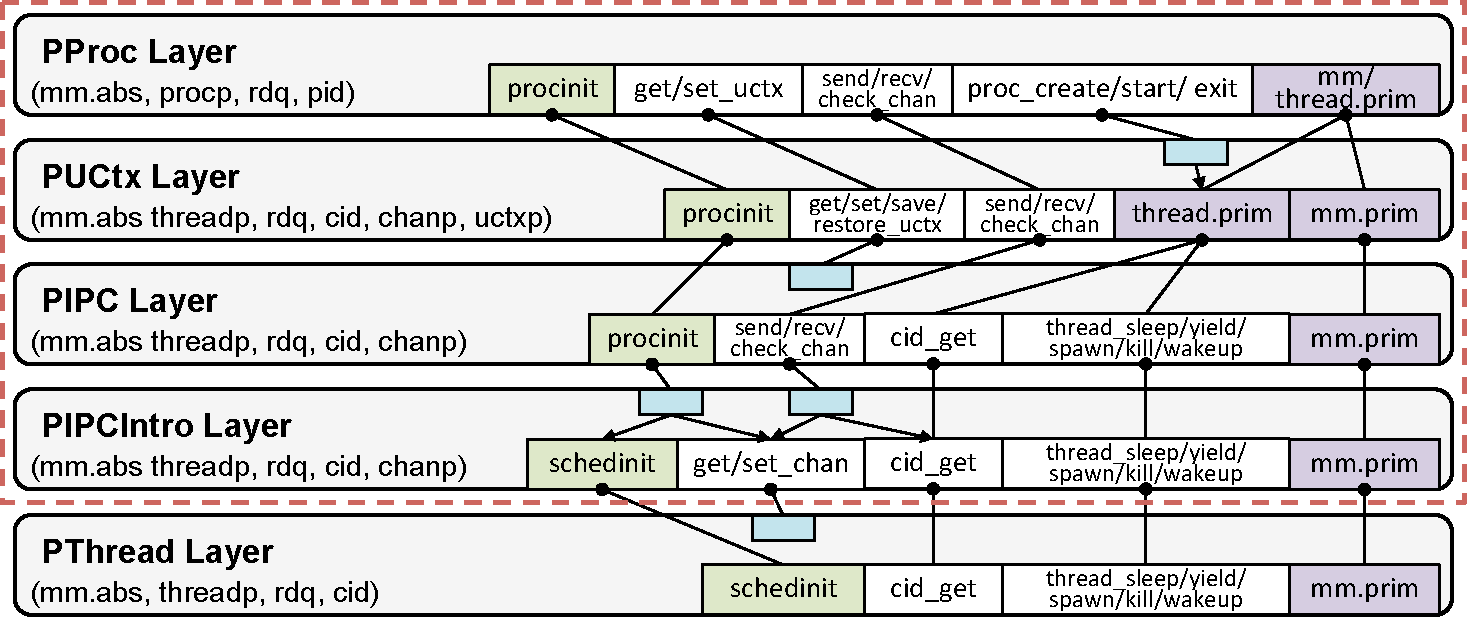
\includegraphics[scale=0.5]{figs/pm_layer}	
\caption{Layers of process management \adam{Missing comma}}
\label{fig:base:pm:layers}
\hrulefill
\end{figure}
}
 
Figure~\ref{fig:base:pm:layers} shows the 4 layers of the process
management module.  The layers \verb"PIPCIntro", and
\verb"PIPC" are the getter-setter layer and abs-kernel-fun layer for
inter-process communication (IPC) channel pool \verb"chanp".  The
layer \verb"PUCtx" is the getter-setter layer for user context pool
\verb"uctxp", while the layer \verb"PProc" introduces
the abstract process pool \verb"procp" and primitives to manage
processes.

In the process management component, we have also implemented and verified a single-copy
synchronous inter-process communication (IPC) protocol.
Additionally, we have verified an
asynchronous zero-copy IPC implementation that is built on top of our
shared memory infrastructure.

\ignore{
As shown in Fig.~\ref{fig:abs:threadproc} (right),
an abstract \verb"process" consists of a kernel thread, a page map,
a user context, and an IPC channel.
}

\subsection{Trap handler}
\label{sec:base:trap}

\begin{figure}[t]\centering
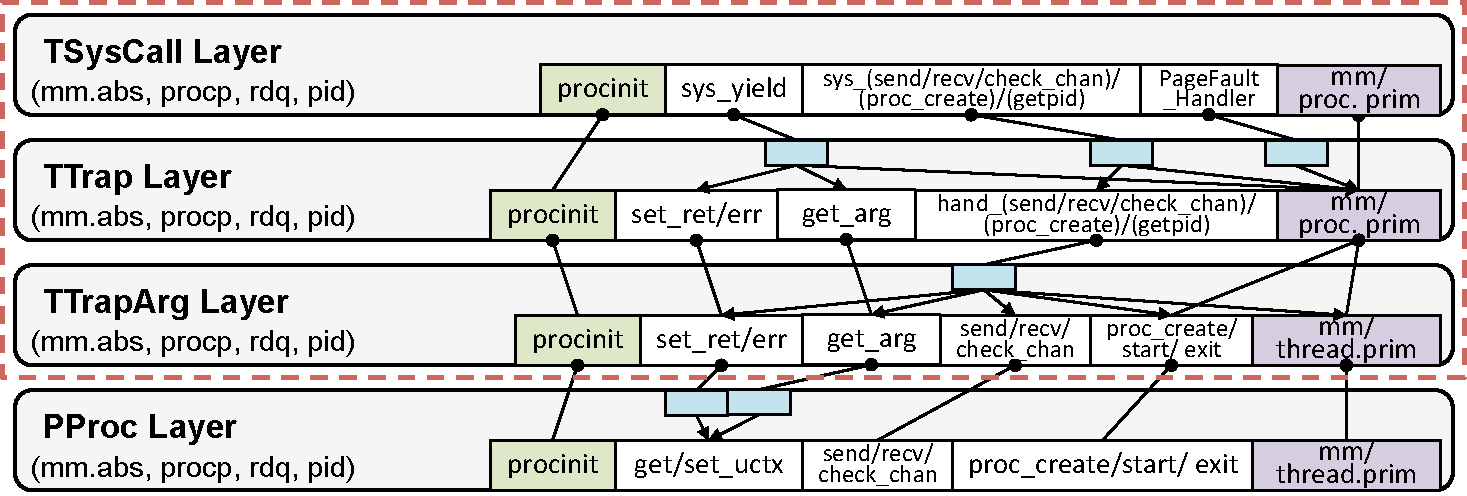
\includegraphics[scale=0.5]{figs/trap_layer_base}	
\caption{Layers of trap handler}
\label{fig:base:trap:layers}
\hrulefill
\end{figure}

{
\begin{figure}\centering
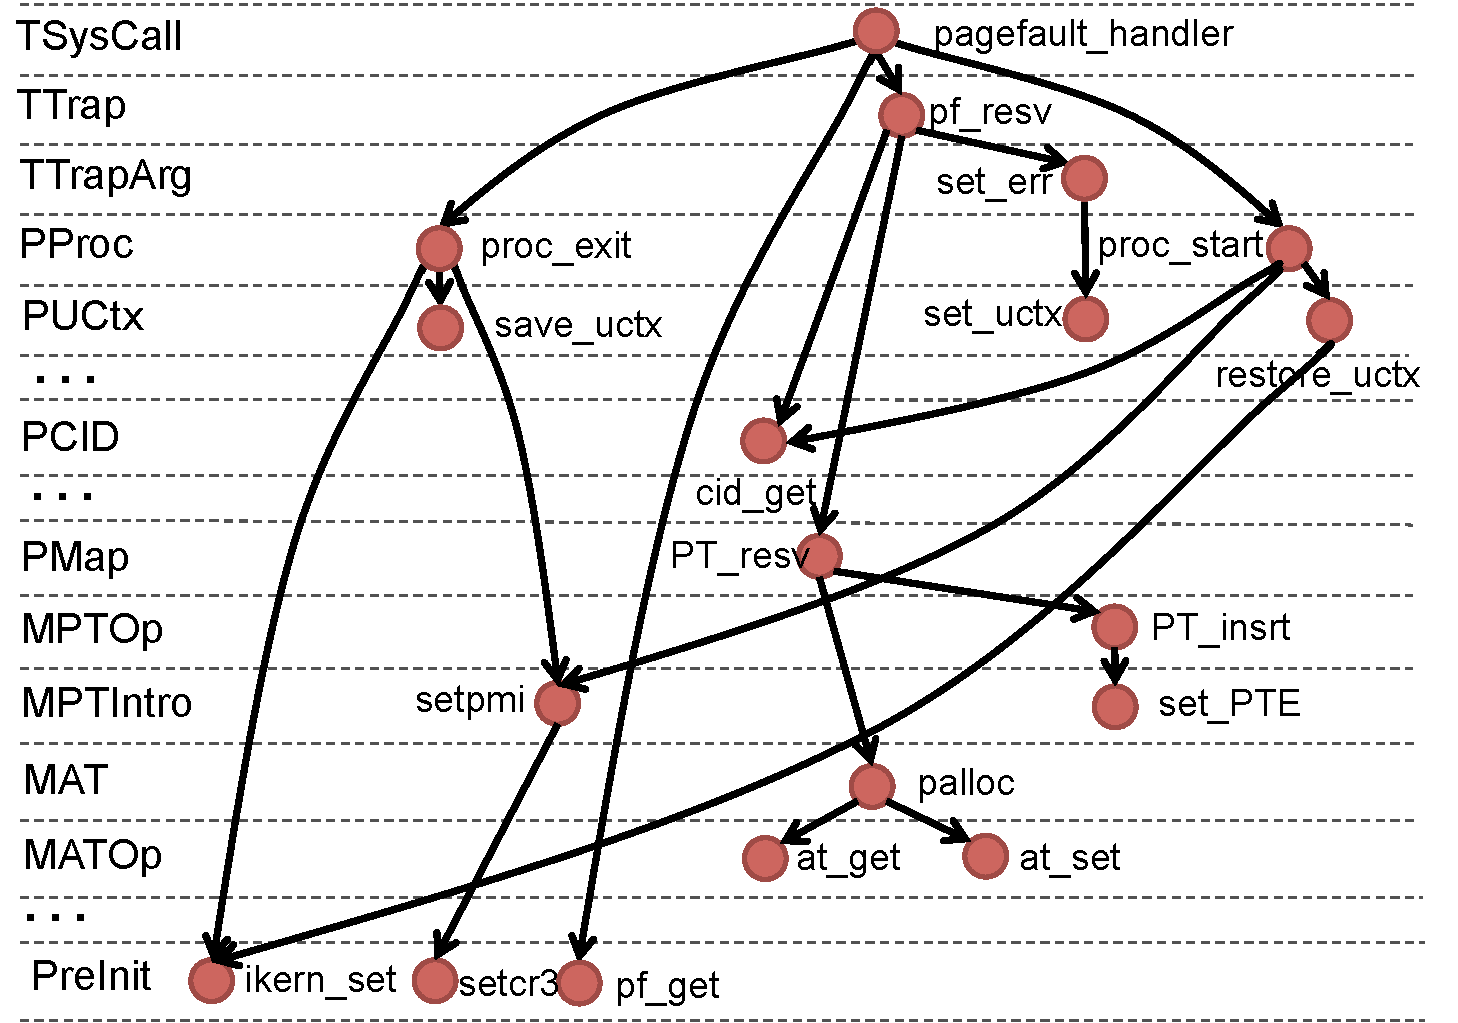
\includegraphics[scale=0.5]{figs/pagefault}	
\caption{Call graph of page fault handler}
\label{fig:base:trap:pagefault}
\hrulefill
\end{figure}
}

The trap module specifies the behaviors of exception handlers and
\mCTOSbase{} system calls.
The trap handler module of \mCTOSbase{} consists of 3 abs-kernel-fun
layers, shown in Figure~\ref{fig:base:trap:layers}.  It specifies the
trap handler module in the standard operating system.  The
\verb"TTrapArg" layer introduces primitives to manage the system call
arguments and return values, while the \verb"TTrap" layer implements
the necessary handlers for system calls and exceptions.  Finally, the
\verb"TSysCall" layer specifies the semantics of system calls from the
user point of view, following the x86 system call convention.

To further simplify the reasoning about user code, we have implemented and
verified the user level system call libraries directly in the user space.
Since our machine semantics models hardware behaviors
like paging and ring switch, the specifications of user system call
libraries closely corresponds to the real execution model in the actual
hardware. With this atomic system call semantics in the user level,
the user code can be proved much more easily.

The behavior that saves and restores the trap frame (user context)
structure is modeled with the primitives \verb"proc_exit" and
\verb"proc_start".  The verified assembly implementation only saves
and restores the second half of the user context as the first half is
saved and restored by the hardware.  

In \mCTOSbase{}, exception handlers are registered in a table of first-class code pointers.
When an exception triggers (via interrupt), the kernel consults this table
and invokes the corresponding exception handler.
For example, a page fault at the user level traps into the kernel.
The page fault handler then reserves a page for PFLA (if necessary)
and returns to the user level.
The verification of the page fault handler depends on layer objects introduced
at different abstraction levels (\cf Figure~\ref{fig:base:trap:pagefault}).
We can see that the
implementation of the page fault handler involves 18 primitives across
12 layers.  On the other hand, the verification of the handler is
fairly simple as it is specified using abstract specifications of the
functions it directly calls on a layer with a very high level of
abstraction (\verb"TTrap").
Therefore, the behavior of the page fault handler is interpreted by
the concrete first-class code pointer until all the dependent layer
objects are introduced.  Then the handler code is verified and
the behavior is interpreted using its abstract atomic specification.


\ignore{
For the exception handler, we
implement the standard page fault handler which dynamically allocates
the user memory in the page table.  Figure~\ref{fig:base:trap:pagefault}
shows the call graph of our page fault handler. 

Here, red
points are primitives at different layers, edges represent
invocations, and the primitives are called from left to right in the
order of the edges. 
}



\ignore{
\subsectskip
\subsection{User-level program}
\label{sec:base:user}
\asubsectskip

Thanks to the contextual refinement relation that we have built between the system call primitives and the underlying kernel implementations, we can reason about the user-level program with the specification of system calls and linked the proof with the one of \mCTOSbase{}.

For example, suppose we have verified that a user process $U$ linked with the system call specifications satisfy the specification $S$, which is
$$
\sem{\rm\mCTOSbase{}}{U}\Refrel{}\sem{}{S}
$$

By the final theorem of \mCTOSbase{} we have proved, 
$$
\forall P,\;\sem{\rm{}x86}{K\join{}P}\Refrel{}\sem{\rm\mCTOS}{P}
$$
, and instantiate $P$ with $U$, we can get the theorem that
$$
\sem{\rm{}x86}{U\join{}K}\Refrel{}\sem{}{S}
$$
, meaning that the user program $U$ linked with the kernel implementation $K$ and running on a x86 bare machine still satisfy the specification $S$.

%% To be moved to POPL: OSDI do not care about C vs. Asm
%%However, one limitation is that, we could not link a certified compiler using flat memory model with \mCTOSbase{}. It means that we can only verify the user-level program at assembly level instead of at C level.

\ronghui{
\begin{itemize}
\item Maybe we can find some interesting user programs
%% \item We can also put the limitation to the section 7. --> moved to POPL
\item where to put the final theorem
\end{itemize}
}
}